\documentclass[11pt]{book}
\usepackage{amsmath,amssymb,amsfonts}
\usepackage{iiit_thesis}
\usepackage{cite}
\usepackage{times}
\usepackage{graphicx}
\usepackage{setspace}
\usepackage{enumitem}
\usepackage{tabularx}
\usepackage{subfigure}
\usepackage{notoccite}
\usepackage{afterpage}
\usepackage{xcolor}
\usepackage{algorithm}
\usepackage{algpseudocode}
\usepackage{multirow}
\usepackage[hidelinks]{hyperref} 
\usepackage[toc,page]{appendix}
\usepackage{comment}
\usepackage{pdfpages}
\usepackage{siunitx}

\graphicspath{{images/}{./}} % To include images in other directories

%------------------------------------------------
% To reduce separation in itemize and enumerate
% \setlist[itemize]{noitemsep} % can include 'nolistsep' also
% \setlist[enumerate]{noitemsep}

%------------------------------------------------
% Settings for Abbreviations and Symbols list
\usepackage[style=super,automake,nogroupskip,nopostdot,symbols,sort=standard,toc=false]{glossaries-extra}
\setglossarystyle{super}
\setabbreviationstyle[acronym]{long-short}
  % \centering
  \renewenvironment{theglossary}%
    {\tablehead{}\tabletail{}%
     \begin{supertabular}{p{4cm}p{\glsdescwidth}}}%
    {\end{supertabular}}%
\makeglossaries
\loadglsentries{acronyms}

%-------------------------------------------------
\long\def\symbolfootnote[#1]#2{\begingroup%
\def\thefootnote{\fnsymbol{footnote}}\footnote[#1]{#2}\endgroup}
\renewcommand{\baselinestretch}{1.2}
\onecolumn
%
\makeatletter
\def\ignorecitefornumbering#1{%
     \begingroup
         \@fileswfalse
         #1%                     % do \cite comand
    \endgroup
}
\makeatother

%-------------------------------------------------
% Custom commands
\newcommand{\p}{\mathbb{P}}
\newcommand{\gt}{\gamma_{\text{th}}}
\newcommand\txtblue[1]{{\color{blue}#1}}
%--------------------------------------------------------

\begin{document}
\pagenumbering{roman}
%% TITLE PAGE
\thispagestyle{empty}
\begin{center}
\vspace*{1.5cm}
{\Large \bf Exploring Gender Disparities in Dating Applications}

\vspace*{2.2cm}
{\large A thesis submitted in partial fulfillment\\}
{\large  of the requirements for the degree of \\}

\vspace*{1cm}
{\it {\large  Master of Sciences} \\
{\large in\\}
{\large Computing and Human Sciences by Research\\}}

\vspace*{0.8cm}
{\large by}

\vspace*{6mm}
{\large Ritvik Aryan Kalra\\}
{\large 2019115002\\
{\small \tt ritvik.kalra@research.iiit.ac.in}}

\vspace*{5mm}
{\large Advisor: Dr. Nimmi Rangaswamy\\}


\vspace*{3.0cm}
{
\includegraphics[width=5cm]{figures/iiit.png}\\}
{\large International Institute of Information Technology Hyderabad\\}
{\large 500 032, India\\}
\vspace*{5mm}
{\large April 2024\\}
\end{center}

%----------COPYRIGHT PAGE--------------------
\newpage
\thispagestyle{empty}
\renewcommand{\thesisdedication}{{\large Copyright \copyright~Firstname Lastname, 2023\\}{\large All Rights Reserved\\}}
\thesisdedicationpage

%------------------------------------------------
\newpage
\thispagestyle{empty}
\vspace*{1.5cm}
\begin{center}
{\Large International Institute of Information Technology Hyderabad\\}
{\Large Hyderabad, India\\}
\vspace*{3cm}
{\Large \bf CERTIFICATE\\}
\vspace*{1cm}
\noindent
\end{center}
This is to certify that work presented in this thesis proposal titled \textit{\textbf{Exploring Gender Disparities in Dating Applications}} by \textit{Ritvik Aryan Kalra} has been carried out under my supervision and is not submitted elsewhere for a degree.

\vspace*{3cm}
\begin{tabular}{cc}
\underline{\makebox[1in]{}} & \hspace*{5cm} \underline{\makebox[2.5in]{}} \\
Date & \hspace*{5cm} Advisor: Dr. Nimmi Rangaswamy 
\end{tabular}
\mastersthesis
% \renewcommand{\baselinestretch}{1.5}
%
% ABSTRACT PAGE
\chapter*{Abstract}
\label{ch:abstract}
Lorem ipsum dolor sit amet, consectetur adipiscing elit. Sed consectetur, tortor ut cursus commodo, leo nisi lacinia orci, in consectetur odio ligula non lectus. Vestibulum vitae enim at libero feugiat finibus. Aliquam vitae malesuada odio. Nullam sed quam vel ex ultricies congue. Vivamus ac elit faucibus, sodales ex id, placerat quam. Quisque tristique dapibus nisl, in vestibulum leo malesuada sit amet. Proin ut augue semper, convallis tellus id, tincidunt nulla. Curabitur eu sollicitudin nisl. Morbi maximus diam eu neque volutpat faucibus. Phasellus non odio dui.

Pellentesque fringilla ante at sem aliquam, sed consequat nisl pharetra. Nullam eu urna vel lectus efficitur maximus. Fusce ut ex eu purus rutrum tempor a sed lectus. Integer ultrices est elit, sed interdum ipsum efficitur in. Sed tristique, mauris eu tempor consectetur, ante massa fringilla risus, sed consectetur mi justo id nisi. Ut tempor luctus mauris sed fringilla. Vestibulum eu elit in turpis iaculis elementum. Aenean nec odio sit amet lorem elementum consequat. Vivamus condimentum metus a turpis consectetur luctus. Integer nec sem eu diam vestibulum tincidunt.

Nam sed mi eu tortor posuere sollicitudin eget ac lacus. Integer suscipit bibendum arcu, at semper leo faucibus non. In vulputate tortor eu neque ultrices, id feugiat tortor condimentum. Aenean vestibulum risus vitae nibh finibus, eget lobortis dolor placerat. Mauris in facilisis nisi. Proin congue auctor nisi, eu bibendum dui bibendum vitae. Fusce vitae arcu id lacus faucibus pretium. Donec quis turpis a metus eleifend finibus nec eget tortor. Curabitur interdum dui mauris, vitae finibus felis viverra in. Quisque eget est vitae nulla hendrerit iaculis. Phasellus pellentesque interdum elit, a finibus nunc iaculis a.
%
\tableofcontents
\listoffigures
\let\cleardoublepage\clearpage
\listoftables
\printglossary[type=\acronymtype,title=Abbreviations,nonumberlist]
\printunsrtglossary[type=symbols]

%--------------------------------------------------------
% % 'List of Publications'
% \chapter*{List of Related Publications}
% \label{ch:relatedPubs}
% \begin{enumerate}[label={[P\arabic*]}]  
    \item Author1, Author2, and Author3, \textbf{``Title of the paper published in the conference or journal"}, in proceedings of {\it IEEE International Symposium on the name of the conference or journal}, 2020.
    
    \item Author1, Author2, and Author3, \textbf{``Title of the paper published in the conference or journal"}, in proceedings of {\it IEEE International Symposium on the name of the conference or journal}, 2020.

    \item Author1, Author2, and Author3, \textbf{``Title of the paper published in the conference or journal"}, in proceedings of {\it IEEE International Symposium on the name of the conference or journal}, 2020.
    
\end{enumerate}
\noindent
Related co-author publications:
\begin{enumerate}[start=3,label={[P\arabic*]}]
    \item Author1, Author2, and Author3, \textbf{``Title of the paper published in the conference or journal"}, in proceedings of {\it IEEE International Symposium on the name of the conference or journal}, 2020.
    
    \item Author1, Author2, and Author3, \textbf{``Title of the paper published in the conference or journal"}, in proceedings of {\it IEEE International Symposium on the name of the conference or journal}, 2020.

\end{enumerate}

%--------------------------------------------------------
\chapter{Introduction}
\label{ch:intro}
The advent of online dating platforms, spearheaded by technological advancements and changing societal norms, has significantly transformed the landscape of romantic and interpersonal relationships. Among these platforms, Bumble has emerged as a frontrunner in India, promoting itself as a site of progressive values with its unique feature allowing only women to initiate conversations \cite{noauthor_bumble_nodate}. This shift towards digital intimacy is underpinned by a growing internet user base in India, projected to reach 1.3 billion in 2023 \cite{noauthor_india_nodate},  creating an expansive arena for online dating applications.

The promise of these platforms, however, is mired in complexities concerning algorithmic biases. Despite their potential for facilitating diverse and inclusive interactions, the algorithms driving these platforms often replicate and amplify societal biases. Such biases are not inherent to the algorithms but stem from the data on which they are trained, reflecting historical and cultural prejudices \cite{davidson-etal-2019-racial, Raghavan_Barocas_Kleinberg_Levy_2019}. In the case of Bumble, the platform's algorithm learns from user behavior to make match recommendations, a process that, while seemingly neutral, can inadvertently perpetuate discrimination based on gender and other social identities. Kordzadeh \& Ghasemaghaei highlight the scant empirical examination of algorithmic bias, despite extensive conceptual discussion of its ethical, legal, and design implications. Their work underscores a critical gap in understanding how biases embedded within algorithms affect user perceptions and behaviors, particularly in systems driven by data and designed to make recommendations, such as online dating platforms.

The consequences of these biases extend beyond the digital space, affecting users' self-perception and interaction with others. For individuals of non-binary genders, these biases can result in a reduced visibility and misrepresentation, reinforcing existing gender norms and excluding them from fully participating in the online dating experience \cite{Bivens_Hoque_2018, MacLeod_McArthur_2019}. The "Elo Score" system, speculated to be used by Bumble, illustrates this issue by ranking desirability based on opaque factors, potentially marginalizing users who do not conform to mainstream criteria of attractiveness \cite{Carr_2016}

Furthermore, the role of dating apps in shaping social norms and behaviors is increasingly acknowledged, with platforms like Bumble influencing not just romantic interactions but also broader societal perceptions of gender and sexuality \cite{Das_2019, Forbes_2020}. The integration of features aimed at inclusivity, such as pronoun selection and guides for queer dating, highlights Bumble's efforts towards creating a safer and more welcoming environment for all users. Yet, the persistence of algorithmic biases underscores the challenges of reconciling technological innovation with the need for social justice and equality.

The study of gender disparities in Bumble's match recommendations thus sits at the intersection of technology, culture, and social justice. It offers a critical lens through which to examine the implications of algorithmic decision-making on social identities, highlighting the urgent need for more inclusive and equitable design practices in the realm of online dating.

\section{Statement of the Problem}
The proliferation of digital platforms has transformed many aspects of human social interaction, notably the sphere of romantic and interpersonal relationships. Among these platforms, dating applications like Bumble have gained prominence for facilitating connections between users. However, these applications are not devoid of implications for social equity and inclusivity. Recent research has underscored the potential for algorithmic bias in such platforms, which can perpetuate and even amplify societal biases, particularly those related to gender \cite{Hutson_Taft_Barocas_Levy_2018, Lambrecht_Tucker_2019, Selbst_Boyd_Friedler_Venkatasubramanian_Vertesi_2019}

This study specifically investigates the problem of gender disparities in the algorithmic recommendations provided by Bumble, a leading dating platform. Bumble’s algorithms, which are designed to learn from user behavior and preferences, may inadvertently reproduce existing societal biases, affecting the visibility and representation of users across the gender spectrum. The gravity of this issue is magnified in the Indian context, where rapid digitalization and shifting cultural norms around gender and relationships create a complex socio-technical landscape \cite{Das_2019, Forbes_2020}.

Despite Bumble's efforts to create an inclusive platform — such as offering extensive gender identity options and promoting women's agency in initiating conversations — concerns remain regarding how the underlying algorithmic processes may favor certain user groups over others \cite{Bivens_Hoque_2018, MacLeod_McArthur_2019}. The preliminary findings from our research suggest a notable discrepancy in the match recommendations for users identifying with different genders, with non-binary users potentially facing distinct challenges \cite{Kalra_Gupta_Varghese_Rangaswamy_2023}.

This problem is situated within a broader discourse on algorithmic fairness, which demands critical scrutiny of the socio-technical systems that increasingly mediate human interactions. The implications of biased algorithmic recommendations extend beyond individual user experiences, reflecting and reinforcing wider social inequities. Thus, this study seeks to articulate and analyze the specific manifestations of gender bias within Bumble's recommendation algorithms and explore their implications for users’ experiences and identities, particularly in the Indian socio-cultural context.

Addressing this problem necessitates a multi-dimensional investigation that considers not only the technical workings of algorithms but also their interaction with human behaviors, societal norms, and the regulatory frameworks that govern digital platforms. By exploring the nuances of gender bias in Bumble’s algorithmic recommendations, this research contributes to the broader discourse on digital ethics, social justice in technology design, and the pursuit of inclusivity in digital spaces.

\section{Research Objectives}
\subsection{Analyze Algorithmic Biases in Match Recommendations}
\textbf{How are gender preferences and identities represented and operationalized within Bumble's algorithmic logic?}
This inquiry focuses on the technical underpinnings of Bumble’s algorithms, seeking to unravel the specific data inputs and machine learning models that might contribute to biased outcomes. By examining the algorithmic criteria that influence match recommendations, this research aims to pinpoint the methodological aspects where biases could be introduced or perpetuated.

\subsection{Understand User Experiences and Perceptions}
\textbf{How do users of different gender identities perceive the impact of algorithmic recommendations on their interactions within Bumble?}
This question aims to capture a broad range of user experiences through qualitative methods, such as interviews and surveys, to understand the subjective dimensions of algorithmic biases. It seeks to identify common themes in user perceptions, including feelings of inclusion or exclusion, the accuracy of match recommendations, and the overall influence on users’ dating experiences.

\textbf{How do these perceptions vary across different cities and socio-cultural contexts within India?}
Recognizing the diversity within India, this question explores regional variations in user experiences, considering how urban and rural settings, as well as cultural differences, might affect the manifestation and perception of biases in Bumble’s recommendations.

\subsection{Examine Social and Ethical Implications}
\textbf{What are the ethical considerations for designing and implementing algorithms in social platforms like Bumble, especially in culturally diverse settings like India?}
This question aims to bridge the gap between technological design and ethical imperatives, considering the responsibilities of developers and platforms in ensuring fairness and equity. It explores the balance between algorithmic efficiency and social justice, questioning how platforms can adhere to ethical guidelines while maintaining their functionality and user appeal.

\subsection{Propose Solutions for Enhancing Fairness and Inclusivity}
\textbf{What design principles and policy measures can be adopted by Bumble and similar platforms to mitigate gender biases and promote inclusivity?}
This question is forward-looking, aiming to translate the findings of the study into actionable recommendations for digital platforms. It considers both technical adjustments, such as algorithmic audits and diversification of training data, and policy interventions, such as transparency measures and user feedback mechanisms.

\textbf{ How can community engagement and user feedback be effectively integrated into the design and continuous improvement of dating apps?}
Recognizing the value of participatory design, this question explores methods for involving users directly in the platform development process, ensuring that diverse perspectives are considered in shaping algorithmic recommendations.

\subsection{Anticipated Impact}
The findings from this study are anticipated to contribute significantly to the fields of social computing, algorithmic fairness, and digital ethics. By providing a nuanced understanding of how gender biases manifest in Bumble’s match recommendations and affecting users’ experiences, this research aims to spark a broader conversation on the need for inclusive design in technology. It seeks to inform developers, policymakers, and the broader community about the critical role of ethical considerations in the development and deployment of algorithms, with the ultimate goal of fostering digital spaces that are equitable and welcoming for all users, regardless of gender identity.

\section{Significance of the Study}
The exploration of gender disparities in Bumble’s match recommendations is a timely and critical inquiry that stands at the intersection of technology, society, and ethics. This study is significant for several reasons:

\begin{itemize}
    \item \textbf{Academic Contribution:} By investigating the nuanced ways in which algorithmic processes may perpetuate gender biases, this research contributes to the burgeoning field of algorithmic fairness. It adds a unique perspective by focusing on a non-Western context, thereby enriching the global discourse on digital ethics and inclusivity. Furthermore, it addresses a gap in existing literature by specifically examining the experiences of non-binary and marginalized gender identities within dating platforms, a topic that remains underexplored. This work will be of interest to scholars in information systems, gender studies, social computing, and human-computer interaction, offering empirical evidence and theoretical insights that can inform future research endeavors.
    \item \textbf{Industry Impact:} For developers, designers, and operators of digital platforms, the findings of this study provide a crucial understanding of the implications of their algorithmic decisions. By highlighting specific areas where biases manifest, this research can guide the development of more inclusive and equitable algorithmic systems. It offers practical recommendations for incorporating ethical considerations into the design and operation of dating apps, encouraging industry stakeholders to prioritize user diversity and fairness.
    \item \textbf{Policy Implications:} This study has the potential to inform policy and regulatory frameworks governing digital platforms. By elucidating the complex dynamics of algorithmic bias and its impact on users, the research supports the development of guidelines and standards that ensure digital inclusivity and protect user rights. Policymakers can leverage the insights gained to advocate for transparency, accountability, and ethical practices in the tech industry, contributing to safer and more inclusive digital environments.
    \item \textbf{Social Awareness:} At a broader level, this research underscores the social responsibility of digital platforms in shaping societal norms and interactions. By examining the impact of gender biases in match recommendations, the study highlights the role of technology in reinforcing or challenging existing social inequalities. It sparks a critical conversation about the need for digital spaces that affirm diverse identities and foster inclusive communities. For users of dating apps and the wider public, the study raises awareness about algorithmic biases and their implications, promoting digital literacy and advocating for equitable technology use.
    \item \textbf{Advancing Inclusivity:} Ultimately, the significance of this study lies in its contribution to advancing inclusivity in digital platforms. By providing a nuanced analysis of gender disparities in Bumble’s match recommendations and offering actionable insights for enhancing algorithmic fairness, this research plays a vital role in promoting a more inclusive digital society. It not only sheds light on the challenges faced by marginalized communities but also charts a path forward for creating digital platforms that are truly reflective of and responsive to the diversity of human experiences.
\end{itemize} 

\section{Scopes and Limiations}
The exploration of gender disparities in Bumble’s match recommendations undertaken in this study is bounded by a focused examination of user experiences across different gender identities within metropolitan areas of India. The choice to center the research on urban settings was informed by the higher prevalence and diverse user engagement with dating apps in these areas, providing a fertile ground for investigating the nuances of algorithmic bias and user interactions. However, the study’s concentration on a small participant pool, while enabling a detailed qualitative analysis of individual narratives, introduces several limitations that must be acknowledged.

Firstly, the findings of this study, owing to its limited geographic focus and sample size, may not encapsulate the breadth of experiences of all Bumble users in India, especially those residing in rural or less urbanized locales. The diversity of socio-cultural norms, access to technology, and attitudes towards gender and dating outside metropolitan areas remains unaddressed, potentially limiting the generalizability of the research outcomes.

Moreover, despite including participants from a range of gender identities, the limited number of participants means the study might not fully represent the extensive spectrum of user experiences related to gender diversity on Bumble. The complexity and individuality of gender identity and expression suggest that a broader, more heterogeneous sample could unveil additional insights into the platform’s inclusiveness.

A significant challenge faced by this research is the proprietary nature of Bumble’s algorithms. The lack of direct access to the algorithmic frameworks and data sets underpinning match recommendations means that any analysis of algorithmic biases is necessarily based on indirect evidence, such as user perceptions and observed outcomes. This limitation underscores the broader issue of algorithmic transparency within digital platforms.

Lastly, the study's findings reflect a particular moment in time, framed by the current state of Bumble’s algorithms, user behaviors, and societal attitudes towards gender and dating. The dynamic nature of digital platforms means that these elements are subject to change, which could affect the relevance of the study’s conclusions in the future.

Despite these constraints, the research provides crucial insights into the presence and implications of gender biases in algorithmic match recommendations on Bumble, highlighting the need for ongoing investigation into algorithmic fairness and inclusivity. It contributes to a deeper understanding of the intersection between technology and social dynamics, laying the groundwork for future research and discussions on creating equitable digital spaces.



%--------------------------------------------------------
\chapter{Literature Review}
\label{ch:literature review}
In the rapidly evolving landscape of India's social and romantic interactions, the surge in online dating platforms like Bumble has marked a significant shift in how relationships are formed and nurtured. This shift, driven by technological advancements and changing cultural attitudes, underscores the critical importance of studying anti-discrimination within these digital realms. As internet usage in India reached an unprecedented 1.3 billion by 2023 \cite{statista_internet_users_2050}, the role of algorithms in shaping social dynamics becomes increasingly pertinent. Our research delves into the complexities of algorithmic bias and discrimination on Bumble, an online dating platform that has gained popularity among Indian users. By integrating insights from AI fairness and inclusion studies, we aim to dissect the algorithmic underpinnings that could perpetuate discrimination in the digital dating scene.

Online dating applications, which involve creating user profiles to search for and communicate with potential partners, have become a cornerstone of modern romantic and social interactions. These platforms employ various technologies, including location-based services and sophisticated algorithms, to suggest compatible partners to users. Specifically, Bumble's recommendation algorithm, which is speculated to utilize an "Elo Score" similar to that of Tinder, plays a pivotal role in this process. This score, a measure of desirability rather than mere attractiveness, is determined by a user's interaction patterns, such as "swipes" on profiles, as well as how other users interact with their profile. Despite the opacity surrounding the exact mechanics of these recommendation engines, it is evident that their effectiveness hinges on the representativeness and quality of the training data used.

However, the deployment of such algorithms raises concerns regarding the potential reinforcement of mainstream content while sidelining diverse and minority perspectives.\cite{davidson-etal-2019-racial} This issue, likely stemming from inadequate representation within the data, leads to a skewed presentation of profiles that disproportionately reflects prevailing societal preferences. The consequent narrowing of content diversity not only reinforces pre-existing cultural biases but also limits the exposure range to a homogeneous set of ideas and individuals. Our investigation into Bumble's algorithm seeks to critically evaluate how these dynamics affect interpersonal interactions and self-presentation on the platform.

Furthermore, our study places a particular emphasis on examining the discrepancies and biases in the recommendations made to individuals of dominant genders, such as men and women, compared to those identifying with non-binary genders. This exploration is crucial for uncovering any inherent algorithmic biases and discussing their broader implications for digital social interactions and inclusivity. By doing so, we aim to illuminate the ways in which digital technologies, through their algorithmic decisions, wield power and influence over social life. As this research progresses, it leads us to ponder deeper questions regarding the intersection of technology, society, and the fabric of our interpersonal relationships. Through this comprehensive analysis, we contribute to the ongoing dialogue on AI fairness and strive to foster a more inclusive digital environment where technology serves as a bridge rather than a barrier to social connectivity and understanding.

%----------------------------------------------
\section{Evolution of Dating and Matrimony Technologies}

\subsection{The West}
The history of dating and matrimony in Western societies has evolved significantly over the centuries, shaped by social, economic, religious, and technological changes. This evolution reflects broader shifts in attitudes toward marriage, gender roles, and social interactions. Pre-19th Century, marriages were arranged for political or economic alliances, and love was not considered as a prerequisite for marriage.  It was in the late 18th century that emotions and love started to play a role in matrimony. Newspapers played a crucial role in this evolution. Initially, matrimonial advertisements in newspapers were straightforward, focusing on the financial and social status of individuals seeking spouses. These ads were practical, aiming to match families for mutual economic benefit rather than love. However, as romantic love became more central to marriage, the nature of these advertisements began to change.

By the late 19th and early 20th centuries, personal ads in newspapers started reflecting the shift towards companionate marriage. These ads became more personal and emotional, with individuals describing their personal qualities, interests, and desires for a compatible partner rather than focusing solely on financial stability or social status. This change indicated a broader societal shift towards valuing emotional compatibility and love as the foundation of marriage.\cite{rothman_hands_1987}

\begin{figure}[t!]
\centering
    \subfigure[]{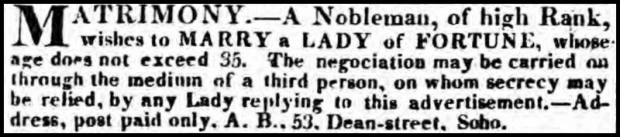
\includegraphics[width=0.45\textwidth]{figures/Introduction/morning-post-june-25-1823.png}\label{fig:img1_a}}\hfill
    \subfigure[]{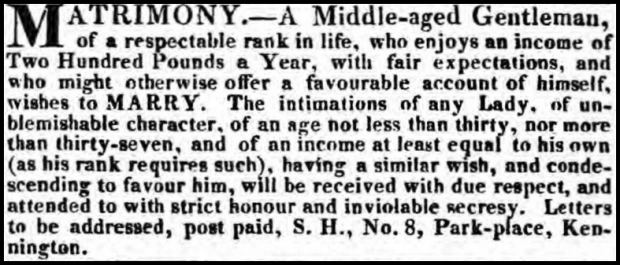
\includegraphics[width=0.45\textwidth]{figures/Introduction/morning-post-december-19-1822.png}\label{fig:img1_b}} 
    \caption{Matrimonial Advertisements in London’s \textit{Morning Post} in the 19th Century}
    \label{fig:img1}
\end{figure}

As the 19th century progressed, the popularity of matrimonial advertisements continued to grow, leading to the emergence of matrimonial specialty magazines like the Matrimonial News and the Matrimonial Intelligencer. These publications were dedicated solely to marriage and complemented the abundance of matrimonial ads found in newspapers, including those targeting specific religious audiences. Religion often played a significant role in these advertisements, highlighting the importance of shared faith in potential matches. Matrimonial ads provided an economical and accessible way for individuals who lacked family, friends, or financial resources to make meaningful connections and seek spouses.\cite{noauthor_alternative_2016}. Figure \ref{fig:img1} shows some of the examples advertisements posted in the newspapers during the 19th century. 

The concept of dating began to take shape at the turn of the 20th century, moving away from the more formal and structured courtship practices of earlier times. Dating became more informal and less focused on immediate marriage, reflecting broader social changes and evolving attitudes toward romantic relationships. This period saw the emergence of "dating" as a distinct phase of a relationship, where couples would spend time together outside the home without the immediate expectation of marriage. This shift was part of a larger cultural change that placed greater emphasis on personal choice and romantic love over social and economic considerations in mate selection. \cite{markarian_how_2017}. In the early 20th century, "Mechanical Matchmaking" emerged, with a notable example being the attempt by Hugo Gernsback, the publisher of Science and Invention magazine, to apply scientific methods to matchmaking. In April 1924, Gernsback proposed four "scientific" tests to determine the likelihood of marital success, including physical attraction tests, sympathy tests, body odor tests, and nervous disorder tests. These methods aimed to quantify and predict the success of marriages, illustrating an early fascination with applying technology and science to personal relationships, much like today's online dating algorithms.\cite{magazine_mechanical_nodate}. In the 1950s, a Newark based, matchmaking service called Introduction, used data as a foundation of their matchmaking services and charged a fee for ‘personalized’ recommendations of suitable matches based on qualifications and social status and subsequent sharing of contact information. \cite{newark_introduction_nodate}

One landmark development in the fusion of technology and dating was Operation Match, which emerged from Harvard University in 1965. Developed by undergraduate students Jeff Tarr and Vaughan Morrill, along with Doug Ginsberg and David Crump, Operation Match was conceived as an innovative solution to the challenges of dating life on campus. Utilizing an IBM 1401 computer, the service employed a sophisticated algorithm to match individuals based on their responses to a comprehensive questionnaire covering personal preferences and interests.\cite{noauthor_operation_1965}  Participants of Operation Match filled out lengthy questionnaires, which they submitted with \$3, and a program on an IBM 1401 computer would match questionnaires to similar responses.\cite{valley_new_2015}  The questionnaires were then transferred to punched cards and processed on an IBM 7090 computer and users received an IBM 1401 print out in the mail a week later, listing the names and contact information of potentially suitable matches. The increased sophistication provided by the IBM 1400 series propelled computer matchmaking into the public shhere as commercial matchmaking servics adopted advanced means to help singles find suitable dates. This increase in popularity of preferenced based match making combined with sexual revolution of the 1960s and 1970s, because of the introduction of oral contraceptives in the 1960s, the rising visibility of the LGBTQ+ community along with the second-wave of feminist movement,\cite{book:1309549} brought upon a drastic change in the attitudes of the people towards dating and relationships. From a culture that only endorsed serious relationships and marriage with the flexibility to choose a sociall equivalent partner, the society started to accept casual dating and hookups. The culture encouraged an individual to explore for their options both sexually and romantically, with multiple partners without any restrictions based on social strata and also having no end goal of marriage. The emergence of modern dating practices offered unprecedented opportunities for social mobility and the exploration of sexuality, albeit within the constraints of the era. This development represented a significant departure from traditional expectations, which often confined individuals to relationships with partners from specific, socially sanctioned groups. Women, in particular, experienced a notable expansion of autonomy through the relaxation of socio-cultural restrictions\cite{book:1309549}. This newfound freedom enabled them to date, form romantic attachments, and partake in sexual relationships with greater agency. 

\begin{figure}[t!]
 \centering
 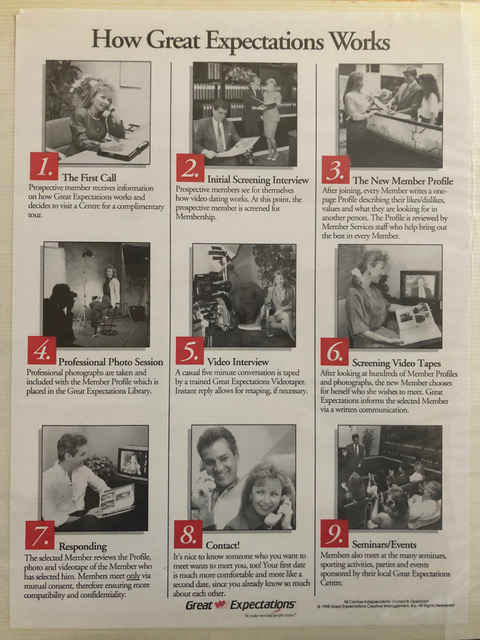
\includegraphics[scale=0.6]{figures/Introduction/GE2.png}
 \caption{A flyer explaining how Great Expectations works}
 \label{fig:img2}
\end{figure}

In the 1980s, post the rise of computer matchmaking, video matchmaking started to emerge. Video (or VHS) dating brought along with it a new way to meet potential partners, with added dimension of being able to hear and see the person before meeting them in person. The first known video dating service was started by Jeffrey Ullman in 1983, called the Great Expectations.\cite{waters_how_2021}. In video matchmaking, participants were asked a series of personal and motivational questions, such as their work ethic, triggers for anger, sources of motivation, and qualities they sought in a partner. After these interviews were recorded, the videotapes were cataloged in a video dating library. Members could browse through this collection, aided by a one-page profile attached to each video that included key details like height, location, and occupation, allowing them to screen potential matches before watching a tape. Figure \ref{fig:img2}, shows a flyer explaining how Great Expectations works. Hearing and Viewing the partners before selecting them was a significant advantage, because as Ullman said ``it showcased a more honest version of a person". \cite{waters_how_2021} This method brought out some of the marvellous personalities of people that would not show up just based on a written questionnaire as was the case in the previous approaches. But the hype of video dating dwindled in the early 1990s because of how cumbersome the process was. It did not bring out a massive change in the dating culture, but it did pave the way for the design of modern dating applications. 

The terminology "matchmaking" is purposefully employed in the preceding sections to delineate pre-Match.com "dating" mechanisms, as these early technologies primarily served the function of facilitating introductions between two parties deemed compatible on a multitude of criteria, ranging from social status to individual predilections and shared ideologies. Prior to the digital revolution instigated by Match.com, "dating" technologies were constrained to the matchmaking domain, enabling initial introductions without encompassing the subsequent phase of dating, which is crucial for assessing compatibility through real-world interactions. The advent of the internet, and specifically Match.com, heralded a paradigm shift by amalgamating matchmaking and dating within a unified online platform. Match.com was instrumental in revolutionizing the dating industry by accelerating the matchmaking process and introducing communication features like chat boxes, thereby allowing matches to engage in preliminary interactions ('date') prior to arranging face-to-face encounters.\cite{noauthor_dating_nodate} This platform introduced the concept of a 'dating profile', encouraging users to provide personal insights alongside photographs, thereby streamlining the process of discovering and interacting with potential matches within a singular service. Contrasting with prior methodologies, which necessitated intermediary involvement and were characterized by significant delays, online dating platforms provided immediate access to an expansive pool of potential matches, along with the autonomy to evaluate compatibility through direct communication, thus enhancing the process's transparency, dynamism, and efficiency.

The evolution of dating technologies further advanced with the development of mobile dating applications, such as Tinder and Bumble, transforming the dating experience into a mobile-centric endeavor. These applications, extensively discussed in the second chapter, innovated user interaction through the implementation of the 'swipe' mechanism and a pronounced focus on visual self-presentation\cite{noauthor_dating_nodate, marcus2016swipe} Notably, such applications significantly contributed to normalizing the sexual exploration or 'hook-up' culture, making it openly accessible and socially acceptable across various demographics\cite{noauthor_dating_nodate, marcus2016swipe}. Tinder, for instance, played a pivotal role in normalizing explicit expressions of sexual intentions by incorporating features that allow users to specify their looking-for preferences, such as casual encounters or long-term relationships, directly on their profiles. Employing sophisticated algorithms and engaging chat functionalities, including emojis, GIFs, and memes, these applications further refined the match screening process, enabling users to make more informed decisions regarding the viability of face-to-face meetings.

This transition from traditional matchmaking services to comprehensive online dating platforms has significantly broadened the interaction spectrum, empowering users to exercise greater selectivity in their dating pursuits. By facilitating a virtual screening process, these digital mediums have not only conserved time and effort but have also expanded the horizons for establishing and nurturing romantic connections in the contemporary era, underscoring a profound shift in the landscape of dating technologies.


\subsection{The Indian Context}
The evolution of dating and matrimony technologies in India has been influenced by the country's unique socio-cultural landscape, characterized by a rich tapestry of traditions, values, and familial structures. It is evident from the previous section that the Western dating culture has undergone significant transformations over the centuries, transitioning from arranged marriages to companionate marriages and subsequently embracing casual dating and hook-up culture. In contrast, to the technologies in the west, dating technology were modified to server as matrimonial services because of the social unacceptability of any form of Dating in the Indian society, until the 2000s \cite{doshi_date_2016, noauthor_modern_2017, sharma_towards_2019}. 

Traditionally, relationships and marriages in India were orchestrated through family networks or arranged by parents, emphasizing communal ties over individual choice. However, the late 20th and early 21st centuries marked a significant transition, driven by technological advancements and a growing emphasis on individual autonomy in choosing romantic partners. Personal advertisements were predominantly utilized to identify appropriate marital alliances, and the inception of Shaadi.com, shortly after the launch of Match.com, mirrored this utility, albeit within the matrimonial context of Indian society. In this cultural milieu, the responsibility of selecting suitable marital candidates traditionally rested with the parents, given the substantial emphasis placed on variables such as caste, religious affiliation, and upbringing. These factors not only held, but continue to hold, considerable importance, with parents extensively relying on their expansive social networks to discover apt matches for their offspring \cite{sharma_towards_2019, seth_online_2008}. Matrimonial services remained largely unchanged, focusing predominantly on matchmaking, as the prerogative to sift through recommended matches was vested in the parents of the concerned individuals, thereby obviating the necessity for incorporating 'dating experiences' to vet multiple prospective partners \cite{titzmann_changing_2013}. The paramount decision-making authority resided with the parents, thus constraining opportunities for dating or romantic exploration—until the widespread adoption of mobile phones in the early 2000s. Mobile telephony and the internet introduced novel avenues for discreet dating, facilitating the quest for partners beyond the traditional constraints of caste and religious affiliations. It is pertinent to highlight that, at this juncture, the Indian dating paradigm mirrored Western practices of the early twentieth century, predominantly aimed at culminating in 'love marriages.'

Liberalization of the Indian economy also played a pivotal role in the introduction of dating applications in India. Liberalization brought upon a transformation in the image of the traditional image of the middle-calss wife India. Traditionally, the middle-class wife in India was emblematic of virtues such as modesty, submissiveness, and a strong adherence to family values, often confined within the domestic sphere and her roles as a caregiver and moral guardian of the family. This portrayal underscored the gender norms and cultural expectations deeply ingrained in the patriarchal fabric of Indian society, where a woman's identity was largely defined through her relationships with men as a daughter, wife, and mother \cite{Dell_2005}.

The onset of economic liberalization introduced a wave of change, marking a pivotal shift in the socio-economic landscape of India. This period was characterized by the opening up of the Indian economy to global markets, an influx of foreign investment, and the adoption of neoliberal policies. Concurrently, this economic shift brought about a significant social transformation, particularly in the roles and perceptions of women in Indian society. The liberalization era ushered in increased educational and employment opportunities for women, challenging the traditional confines of their roles within the household and promoting a narrative of economic empowerment and independence for women. This marked departure from traditional roles was not merely an economic transition but also a cultural shift, fostering a reevaluation of gender dynamics and the emergence of new models of femininity and partnership inspired by global media and the internet \cite{Forbes_2020}.

The increased visibility of women in the workforce and their active participation in public and political spheres echoed the growing feminist movements in India. These movements advocated for gender equality, challenging the patriarchal status quo and pushing for legal and social reforms to address gender discrimination, marital rights, and issues of domestic violence. The discourse around marriage and relationships also evolved, reflecting a gradual shift towards mutual respect, companionship, and shared responsibilities between partners. The liberalization era, therefore, not only transformed the economic landscape but also significantly impacted the social fabric of India, reshaping traditional notions of womanhood and partnership \cite{statista_internet_users_2050}.

In the realm of dating and relationships, the impact of liberalization was further evidenced by the growing acceptance of love marriages, inter-caste and inter-religious unions, and the concept of dating itself—practices once considered taboo. 

The landscape of Indian dating culture witnessed a profound transformation in 2011 with Tinder's entry into the Indian market. Marketed primarily as a 'hook-up' application, Tinder swiftly gained traction among the youth, thereby democratizing dating and, notably, casual romantic encounters. The prevailing narratives suggest a gradual shift from a staunchly arranged marriage-oriented society towards a more open acceptance of 'dating' among the younger demographic. This cultural evolution is fostering the emergence of varied dating practices, spanning from serious relationships to casual dating and hook-ups. The locus of choosing a partner is increasingly transitioning from parents to the individuals themselves, buoyed by the rising popularity of online dating platforms such as OkCupid and Tinder. This paradigm shift towards individual agency in partner selection is a relatively recent development, with online dating gaining the quickest acceptance among college students and young professionals \cite{doshi_date_2016}.

The introduction of dating applications such as Tinder, OkCupid, and Bumble marked a significant cultural shift, offering an alternative to the traditional pathways to marriage. These platforms provided a space for individuals to explore romantic relationships without the immediate objective of marriage, thereby allowing for greater personal autonomy in matters of love and partnership \cite{Das_2019}. his shift is reflective of a broader global trend where individual choice and compatibility are increasingly valued over traditional matchmaking criteria.

The Chief Marketing Officer of OkCupid highlighted the unique nature of the Indian market, noting that a generation of young Indian women is redefining relationship norms by asserting their right to choose their partners. This sentiment encapsulates the transformative impact of dating apps, empowering individuals, especially women, to exercise greater control over their romantic lives "What makes India different is that we have a generation of young women who are changing things by saying, ‘I want to decide who I’m with’" \cite{Forbes_2020}.

In response to the cultural and societal nuances of the Indian context, homegrown applications like TrulyMadly and Aisle have emerged, blending traditional values with modern dating practices. These platforms are designed to cater to the Indian audience's preferences, striking a balance between casual dating and the pursuit of long-term partnerships. By incorporating cultural sensibilities into their algorithms and features, these apps offer a "middle ground" that respects the societal norms and expectations prevalent in Indian society \cite{Forbes_2020}. Bumble, in particular, has made a notable impact by emphasizing women's empowerment through its unique feature that allows only women to initiate conversations.\cite{noauthor_bumble_nodate} This approach not only challenges traditional gender dynamics but also promotes a safer and more respectful online dating environment for women, aligning with broader movements for gender equality and women's rights in India. The rise of dating applications in India is emblematic of the country's ongoing negotiation between tradition and modernity. As India continues to evolve socially and economically, these platforms reflect and facilitate changing attitudes towards relationships, marriage, and personal autonomy. Moreover, the success and adaptation of these platforms in India underscore the globalized nature of technological and cultural exchange, where Western innovations are localized to fit the specific needs and contexts of different societies.

The embrace of Bumble's features by women in India marks a notable shift in the country's dating culture. Women making the first move over 15 million times and sending twice the number of messages compared to the global average highlights a significant change in gender dynamics within the dating scene. This statistic not only signifies women's acceptance of the platform but also their active engagement in shaping their romantic interactions, which is a departure from the traditionally passive role attributed to women in the courtship process in India (Hindustan Times, 2020).

Moreover, the fact that 32\% of women users in India use more than one mode on Bumble suggests that the app is being used not just for dating but also for forming broader social connections. This indicates a broader application of the app's features, possibly extending to networking and friendship, reflecting a versatile use of technology to fulfill various social needs \cite{HindustanTimes_2020}. Further emphasizing the influence of contemporary culture on dating preferences, a recent Bumble report highlights how social media, music, food, literature, and content consumption are shaping Gen Z's dating ideals in India. These factors are indicative of a more globalized approach to dating where personal interests and cultural consumption significantly influence romantic connections \cite{Chronicle_2023}.

Additionally, changes in dating preferences show a trend towards virtual dating, with predictions that 40\% of single Indians will favor this mode of interaction. This reflects a growing comfort with digital interactions and an appreciation for the importance of education, career choices, and compatibility as bases for forming relationships, beyond just physical or geographical proximity \cite{MediaInfoline_2021}. The integration of technology into personal relationships is not unique to India. Globally, dating apps have reshaped social interactions. For instance, in the United States, Tinder and similar apps have significantly influenced dating norms, with studies indicating that online interactions have become a primary way young people connect romantically and socially. These platforms provide a space where users can express themselves in ways that may not be possible in their immediate physical environments, thus expanding their social horizons \cite{Smith_2016}.

The introduction of Bumble in India has marked a significant development in the visibility and social acceptance of LGBTQIA+ identities within the country. The platform’s proactive stance on inclusivity and safety has played a crucial role in not just providing a dating service but also advocating for the rights and recognition of LGBTQIA+ individuals in a society where their acceptance remains inconsistent. The decriminalization of gay sex by the Supreme Court of India in 2018 \cite{Johar} was a landmark moment, legally abolishing Section 377, a colonial-era law that criminalized homosexual acts. However, legal acceptance does not automatically translate into social acceptance, and the LGBTQIA+ community continues to face various forms of discrimination and stigma. In this context, platforms like Bumble serve as important spaces for safe social interaction and self-expression for LGBTQIA+ individuals.

Bumble has introduced several features aimed specifically at enhancing the safety and inclusivity of its platform for LGBTQIA+ users:

\begin{itemize}
    \item \textbf{Guides for Queer Dating:} Bumble provides tailored guides that offer advice and support for queer dating, addressing the unique challenges faced by LGBTQIA+ individuals in navigating the dating world. \cite{Bumble}
    \item \textbf{Incognito Mode:} This feature allows users to maintain privacy and control over who sees their profile, giving LGBTQIA+ users the discretion they may need in a conservative society. \cite{Bumble_incognito}
    \item \textbf{Private Detector:} Bumble’s private detector automatically blurs lewd images to protect users from unsolicited explicit images, enhancing the safety of interactions. \cite{Bumble_private_detector}a
    \item \textbf{Photo Verification:} This feature helps to ensure that profiles are genuine, reducing the risk of catfishing and improving trust and safety on the platform. \cite{Bumble_photo_verification}
    \item \textbf{Pronoun Selection:} By allowing users to select and display their pronouns, Bumble fosters an environment of respect and recognition for gender identity, which is particularly important for transgender and non-binary individuals. \cite{Bumble_pronoun_feature}
\end{itemize}

Bumble’s efforts extend beyond individual safety to influence broader social perceptions and norms regarding LGBTQIA+ identities. By normalizing the inclusion of diverse sexual orientations and gender identities in its platform, Bumble challenges societal prejudices and promotes greater visibility and acceptance of the LGBTQIA+ community. This visibility is crucial in changing public attitudes and encouraging more open discussions about LGBTQIA+ issues in India. Research on the impact of dating apps on LGBTQIA+ communities indicates that such platforms can significantly affect users' lives by providing spaces for identity exploration and community building that are often unavailable in other areas of their lives. Studies suggest that dating apps can help lower barriers to social interaction and empower users by allowing them to seek out connections on their own terms \cite{Blackwell_2015}. Moreover, the role of technology in shaping cultural and social dynamics is increasingly recognized, with scholars arguing that digital platforms can play a transformative role in challenging traditional norms and advocating for marginalized communities \cite{Publishers_Distributors4753/23_Road_Delhi}.

\section{Fairness in AI systems}
The widespread adoption of recommendation algorithms across digital platforms, ranging from online shopping to social media, has sparked a growing awareness of their capacity to perpetuate social injustices. These algorithms are fundamental in shaping user experiences by predicting and influencing behavior through the processing of vast datasets. However, despite their utility, they frequently mirror and even magnify existing societal biases, embedded unintentionally within the data they analyze. This issue arises from algorithms learning from real-world data that reflects historical inequalities or prevalent stereotypes, leading to decisions that systematically disadvantage certain groups.

The inadvertent reinforcement of biases by algorithms not only affects the fairness of automated decisions but also raises ethical concerns about the integrity of AI systems in various applications. As these systems become more integral to everyday life, the urgency for addressing these biases grows, necessitating a careful examination of how algorithms interact with societal norms and structures. Researchers have argued for the development of methods to detect and mitigate biases in AI systems as a critical step towards ensuring they promote equity and fairness. The challenge lies in the inherent complexity of AI models and the subtlety with which biases can be integrated into algorithmic decisions, often masked by the technical opacity of these systems.

Significant scholarly attention has been directed towards understanding the scope and impact of algorithmic bias. Studies have consistently highlighted the need for transparency in AI processes and the implementation of robust fairness metrics to evaluate and rectify biases. The push towards ethical AI involves a multidisciplinary approach, incorporating insights from computer science, social sciences, and legal studies to create AI systems that are not only effective but also equitable and just.

Therefore, addressing these challenges is not merely a technical task but a societal imperative, requiring concerted efforts from developers, regulators, and users alike. Ensuring the fairness of AI systems is fundamental to harnessing the full potential of this technology in a way that benefits all sections of society equitably, fostering trust and wider acceptance of AI applications across various domains.

In recent years, numerous cases have highlighted the inherent risks of discrimination and biases embedded in AI systems, particularly those used in recommendation engines and automated decision-making. These issues not only raise ethical concerns but also underscore the need for more robust frameworks to ensure fairness in AI deployments.

\subsection{Racial Bias in Judicial Algorithms}
One of the most notable instances of AI bias is seen in the COMPAS algorithm, used in the criminal justice system in the United States. This algorithm was found to misclassify black defendants as having a higher risk of reoffending compared to their white counterparts, leading to unfairly harsher sentencing and bail decisions. This case underscored the racial biases that can be perpetuated by automated systems, raising alarms about the fairness and impartiality of using AI in legal contexts \cite{Mattu}.

\subsection{Gender Bias in Job Advertisements}
Another significant example is the gender bias in job advertising on platforms like Facebook, where algorithms were found to display ads for high-paying job opportunities more frequently to men than to women. This was not the result of explicit programmer intent but rather the outcome of the algorithm learning from existing societal biases, indicating that without careful oversight, AI systems can reinforce and perpetuate existing inequalities \cite{Lambrecht_Tucker_2019}.

XING, a professional networking and job recruitment platform similar to LinkedIn, has also faced scrutiny for biases in its job recommendation algorithms. A notable instance of this was highlighted in a study that found XING's algorithms recommended more underqualified men for certain jobs than qualified women. This disparity suggests the presence of gender bias within the algorithm's decision-making processes.

The study indicated that such biases could stem from the training data used to develop these algorithms. If the historical data on which these systems are trained contain gender imbalances—for instance, more men being hired for certain types of jobs than women—algorithms may inadvertently learn to perpetuate these patterns. This results in a feedback loop where men continue to be favored over equally or more qualified women, reinforcing gender inequality in professional settings.\cite{Lahoti_Gummadi_Weikum_2019}

\subsection{Bias in Mortgage Applications}
AI systems have also been implicated in biases affecting mortgage approval processes. Research has shown that automated algorithms used by financial institutions to determine eligibility for loans were less likely to approve loans for applicants from minority backgrounds compared to similar white applicants. This kind of financial bias has significant long-term impacts on wealth accumulation and equality in access to housing \cite{Bartlett_Morse_Stanton_Wallace_2022}

\subsection{Bias in Facial Recognition Technologies}
Facial recognition technologies, widely used in surveillance and security applications, have been criticized for their higher rates of misidentification among people of color, particularly black individuals, and women. This not only raises privacy concerns but also poses a risk of wrongful accusations in law enforcement and security settings. Studies have shown that these biases are due to the underrepresentation of these groups in the training datasets used to develop these technologies \cite{Buolamwini_Gebru_2018}

\subsection{Ethical Concerns in Healthcare Algorithms}
In healthcare, algorithms designed to predict patient health outcomes and allocate healthcare resources have shown biases against certain demographic groups. For example, an algorithm widely used in U.S. hospitals was found to be biased against black patients in its predictions of healthcare needs, resulting in less healthcare resources being allocated to black patients compared to white patients with similar conditions. \cite{Obermeyer_Powers_Vogeli_Mullainathan_2019}

%--------------------------------------------------------

\chapter{Conclusion}
\label{ch:conc}
Lorem ipsum dolor sit amet, consectetur adipiscing elit. Sed consectetur, tortor ut cursus commodo, leo nisi lacinia orci, in consectetur odio ligula non lectus. Vestibulum vitae enim at libero feugiat finibus. Aliquam vitae malesuada odio. Nullam sed quam vel ex ultricies congue. Vivamus ac elit faucibus, sodales ex id, placerat quam. Quisque tristique dapibus nisl, in vestibulum leo malesuada sit amet. Proin ut augue semper, convallis tellus id, tincidunt nulla. Curabitur eu sollicitudin nisl. Morbi maximus diam eu neque volutpat faucibus. Phasellus non odio dui.

Pellentesque fringilla ante at sem aliquam, sed consequat nisl pharetra. Nullam eu urna vel lectus efficitur maximus. Fusce ut ex eu purus rutrum tempor a sed lectus. Integer ultrices est elit, sed interdum ipsum efficitur in. Sed tristique, mauris eu tempor consectetur, ante massa fringilla risus, sed consectetur mi justo id nisi. Ut tempor luctus mauris sed fringilla. Vestibulum eu elit in turpis iaculis elementum. Aenean nec odio sit amet lorem elementum consequat. Vivamus condimentum metus a turpis consectetur luctus. Integer nec sem eu diam vestibulum tincidunt.

Nam sed mi eu tortor posuere sollicitudin eget ac lacus. Integer suscipit bibendum arcu, at semper leo faucibus non. In vulputate tortor eu neque ultrices, id feugiat tortor condimentum. Aenean vestibulum risus vitae nibh finibus, eget lobortis dolor placerat. Mauris in facilisis nisi. Proin congue auctor nisi, eu bibendum dui bibendum vitae. Fusce vitae arcu id lacus faucibus pretium. Donec quis turpis a metus eleifend finibus nec eget tortor. Curabitur interdum dui mauris, vitae finibus felis viverra in. Quisque eget est vitae nulla hendrerit iaculis. Phasellus pellentesque interdum elit, a finibus nunc iaculis a.

%--------------------------------------------------------
\bibliographystyle{IEEEtran}
\bibliography{IEEEabrv,cite.bib}{}

% %--------------------------------------------------------
% % 'Publication 1'
% \chapter*{Publications}
% \chapter*{Publication 1}
% \addtocontents{toc}{\protect{\addvspace{3.0ex plus 1pt}}}
% \addcontentsline{toc}{chapter}{\protect{Publication 1}}
% \input{sections/paper1.tex}
% \includepdf[pages={-}]{papers/paper1.pdf}
% %
% %--------------------------------------------------------
% % 'Publication 2'
% \chapter*{Publication 2}
% \addtocontents{toc}{\protect{\addvspace{3.0ex plus 1pt}}}
% \addcontentsline{toc}{chapter}{\protect{Publication 2}}
% \input{sections/paper2.tex}
% \includepdf[pages={-}]{papers/paper2.pdf}

\end{document}
